\documentclass[tikz,10pt,a4paper]{article}
\usepackage[utf8]{inputenc}
\usepackage[edges]{forest}
\definecolor{foldercolor}{RGB}{124,166,198}
\tikzset{pics/folder/.style={code={%
			\node[inner sep=0pt, minimum size=#1,](-foldericon){};
			\node[folder style, inner sep=0pt, minimum width=0.3*#1, minimum height=0.6*#1, above right, xshift=0.05*#1] at (-foldericon.west){};
			\node[folder style, inner sep=0pt, minimum size=#1] at (-foldericon.center){};}
	},
	pics/folder/.default={20pt},
	folder style/.style={draw=foldercolor!80!black,top color=foldercolor!40,bottom color=foldercolor}
}
\forestset{is file/.style={edge path'/.expanded={%
			([xshift=\forestregister{folder indent}]!u.parent anchor) |- (.child anchor)},
		inner sep=1pt},
	this folder size/.style={edge path'/.expanded={%
			([xshift=\forestregister{folder indent}]!u.parent anchor) |- (.child anchor) pic[solid]{folder=#1}}, inner xsep=0.6*#1},
	folder tree indent/.style={before computing xy={l=#1}},
	folder icons/.style={folder, this folder size=#1, folder tree indent=3*#1},
	folder icons/.default={12pt},
}
\usepackage[T1]{fontenc}
\usepackage{amsmath}
\usepackage{amsfonts}
\usepackage{amssymb}
\usepackage{graphicx}
\usepackage{caption}
\usepackage{subcaption}
\usepackage[cache=false]{minted}
\usepackage[obeyspaces]{url}
\usepackage{hyperref}
\hypersetup{
	colorlinks=true,
	linkcolor=blue,
	filecolor=magenta,      
	urlcolor=cyan,
	pdftitle={Overleaf Example},
	pdfpagemode=FullScreen,
}
\title{Cellpose segmentation}
\author{Rémy Torro}

\begin{document}
	\maketitle
	\section{Introduction}
	In this report, we will outline the process of training a Cellpose model from scratch to perform a segmentation task on our own multichannel data. Our example will be paired brightfield and RICM images, for which we want to segment accurately the adhesion patch of adhered cells and pinpoint the location of non-adhered cells. 
	\subsection{Data preparation}
	\begin{figure}[h!]
		\centering
		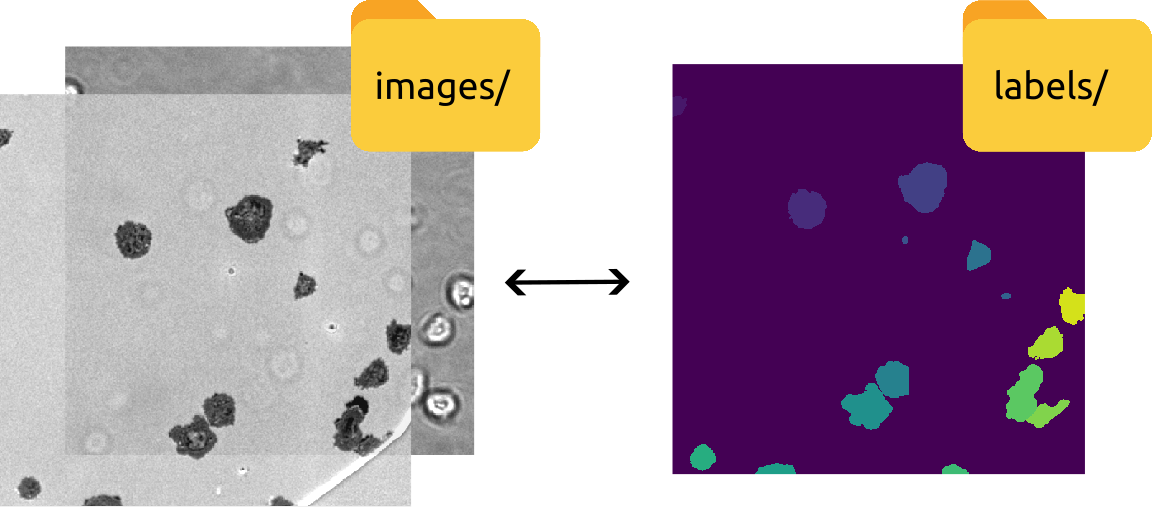
\includegraphics{dataset.png}
		\caption{Example of annotation for one training image. The adhered cells are outlined as precisely as possible whereas non adhered cells only have a very small patch.}
	\end{figure}
	Cellpose expects a training directory and an optional test directory. These directories should contain both the images and the paired annotations. One can specify a suffix for the annotations (\mintinline{bash}{--mask_filter} in the CLI command). Following good practice in Deep Learning, we will perform some data augmentation on our dataset and clearly separate training and testing data. We will export the images with the proper Cellpose-friendly structure of test and train sets.
	
	\subsubsection{Dataset splitting}
	
	\par{} We take at random 25 \% of our dataset as test data. These images and paired annotations are copied to a \path{dataset/test/} folder. No augmentation is performed on the test set. 
	
	\par{} For the remaining images, we will sample, transform and export to the \path{dataset/train/} folder. The transformations include random flipping, random shift, slight intensity fluctuations and a white noise. We re-sample as many time as needed, to give enough inputs to the Cellpose model (here $M = N_{\textrm{train}} \times 2$). 
	
	As a result, the test set contains only original images and the paired annotations, whereas the train sets contains transformed images and the associated annotations. The quantity of train images can exceed the number of images in our dataset. 
	\begin{figure}
	\begin{subfigure}{.5\textwidth}
	  \begin{forest}
		for tree={font=\sffamily, grow'=0,
			folder indent=1.8em, folder icons,
			edge=densely dotted}
		[Original dataset
		[\hspace{3pt} images/, this folder size=10pt
		[im0.tif, is file]
		[im1.tif, is file]
		[im3.tif, is file]
		[..., is file]
		]
		[\hspace{3pt} labels/, this folder size=10pt
		[im0\_labelled.tif, is file]
		[im1\_labelled.tif, is file]
		[im3\_labelled.tif, is file]
		[..., is file]
		]
		]
	\end{forest}
	\caption{Original dataset}
	\end{subfigure}
	\begin{subfigure}{.5\textwidth}
	\begin{forest}
		for tree={font=\sffamily, grow'=0,
			folder indent=1.8em, folder icons,
			edge=densely dotted}
		[Cellpose dataset
		[\hspace{3pt} train/, this folder size=10pt
		[im0\_aug.tif, is file]
		[im0\_aug\_labelled.tif, is file]
		[im1\_aug.tif, is file]
		[im1\_aug\_labelled.tif, is file]
		[..., is file]
		]
		[\hspace{3pt} test/, this folder size=10pt
		[im3.tif, is file]
		[im3\_labelled.tif, is file]
		[..., is file]
		]
		]
	\end{forest}
	\caption{Cellpose-friendly structure}
	\end{subfigure}
	\caption{from the original dataset structure, convenient to annotate many images over many days to a structure directly compatible with the Cellpose CLI command.}
	\end{figure}
	
	\subsubsection{Train Cellpose model}
	
	Once the dataset structure is established, we can use the command line to call for a Cellpose training. A minimum Cellpose CLI command would look like this: 

	\begin{minted}[breaklines,autogobble]{bash}
python -m cellpose --use_gpu --train --dir dataset/train/
	\end{minted}
	
	We run Cellpose in training mode with the flag \mintinline{bash}{--train}, using the GPU with \mintinline{bash}{--use_gpu}, and we point toward the training set with \mintinline{bash}{--dir dataset/train/}. 

	There are more underlying flags that are set to their default value. Let's go step by step towards refining the command to the problem at hand. We introduced a test set, which can be presented to the model with the flag \mintinline[breaklines]{bash}{--test_dir dataset/test/}. 
	We put the \path{_labelled} suffix to the name of the labels. We can pass the flag \mintinline{bash}{--mask_filter} \mintinline{bash}{_labelled}. The images are already normalized, so we pass \mintinline{bash}{--no_norm}, to prevent Cellpose from applying a percentile normalization with clipping. Finally, and most importantly, we have to pass the two channels as inputs (the default will only read the channel interpreted as gray). Standard Cellpose is structured for either:
	\begin{itemize}
		\item a unique cytoplasm channel (\mintinline{bash}{--pretrained_model cyto})
		\item a cytoplasm channel plus a nucleus channel (\mintinline{bash}{--pretrained_model cyto2})
	\end{itemize}

	Since the core of Cellpose is a UNET, we can technically pass any number of channel as the input, without having to make changes to the output. To enter this mode, we have to pass \mintinline{bash}{--pretrained_model None}, and \mintinline{bash}{--all_channels} instead of \mintinline{bash}{--chan 0}. 
	
	Eventually, we end up with a CLI command as follows:
	
	\begin{minted}[breaklines,autogobble]{bash}
python -m cellpose --use_gpu --train --dir dataset/train/ --test_dir dataset/test/ --learning_rate 0.001 --weight_decay 0.01 --n_epochs 5000 --mask_filter _labelled --verbose --no_norm --batch_size 8 --all_channels --pretrained_model None --save_every 100 --save_each
	\end{minted}
	
	The model will train for 5000 epochs and save its weights each 100 epochs. We wil keep each of those intermediate models to compare performance in post.
	
	\subsection{Quality control: selecting the best model}
	
	We can reload any of the intermediate models as follows:
	
	\begin{minted}[breaklines]{python}
from cellpose.models import CellposeModel

model = CellposeModel(gpu=True, 
		    model_type=None, 
		    pretrained_model="path/to/model/",
		    diam_mean=30.0, 
		    nchan=2,
		    )
	\end{minted}

	

\end{document}
